\subsection[Представление генетической информации в электронном виде]{\large Представление генетической информации в электронном виде}
\hspace{\parindent} Поскольку различных нуклеотидов и стандартных аминокислот немного, для их кодирования используют один символ --- первую букву из названия. С другой стороны, названия многих аминокислот начинаются с одинаковых букв, поэтому для кодирования приходится использовать те, которые остаются незанятыми.

\subsubsection[Формат FASTA]{\large Формат FASTA}
\hspace{\parindent} В формате FASTA~\cite{FASTAformat} строчка, начинающаяся с символа '>', называется строкой описания. Она содержит имя последовательности и некоторую дополнительную информацию, предназначенную для идентификации. Другие строки, начинающиеся с символа ';', являются комментариями и игнорируются. За строкой описания следует код последовательности. При кодировании нуклеотидов буквами A, C, G, T и U кодируют, соответственно, аденин, цитозин, гуанин, тимин и урацил. Обычно, длинные последовательности разбивают на несколько строк длиной не более 80 символов --- это не правило формата, но представление данных таким образом выглядит более наглядно для человека.

\subsubsection[Формат FASTQ]{\large Формат FASTQ}
\hspace{\parindent} FASTQ --- формат представления биологической последовательности совместно с данными о качестве. Он используется для представления данных секвенирования. При кодировании уровней качества используются символы из таблицы ASCII от '!' до '\textasciitilde'.\\
\indent Существует два различных способа выражать уровень качества через вероятность ошибки: формулы~\ref{eq:FASTQ:quality1} и~\ref{eq:FASTQ:quality2}, где $Q$ --- уровень качества, а $p$ --- вероятность, что элемент последовательности ошибочный. При малых значениях $p$ эти способы дают практически идентичные результаты, но с ростом $p$ уровни качества начинают заметно различаются (рисунок~\ref{ris:FASTQscore}).

\begin{equation} \label{eq:FASTQ:quality1}
Q = -10 \cdot \log_{10} p
\end{equation}
\begin{equation} \label{eq:FASTQ:quality2}
Q = -10 \cdot \log_{10} \dfrac{p}{(1-p)}
\end{equation}
\begin{figure}[h]
	\center{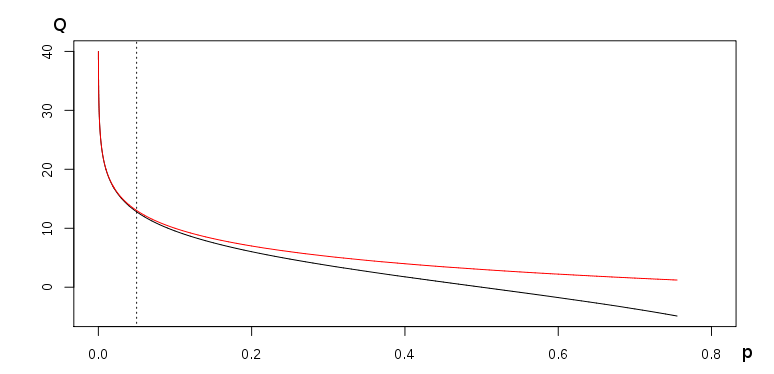
\includegraphics[width=0.9\linewidth]{FASTQscore.png}}
	\caption{График уровней качества для формул~\ref{eq:FASTQ:quality1} (красная) и~\ref{eq:FASTQ:quality2} (черная)}
	\label{ris:FASTQscore}
\end{figure}

\indent Файл в формате FASTQ содержит четыре строки для каждой последовательности. Первая строка начинается с символа '@', после которого идет описание последовательности (строка описания). Следующая строка содержит набор символов, кодирующих саму последовательность аналогично формату FASTA. За ней идёт строка, начинающаяся с символа '+', содержащая дополнительное описание последовательности. Последняя строка содержит уровни качества. 

\subsubsection[Формат GenBank]{\large Формат GenBank}
\hspace{\parindent} Запись в формате GenBank состоит из двух секций: секции аннотации и секции данных~\cite{GenBankFormat}. В первой хранится всевозможная информация о последовательности: из какого организма получена, ссылки на другие работы, различные примечания, а во второй --- сама последовательность, аналогично формату FASTA. Начало секции аннотации отмечается кодовым словом <<LOCUS>>, а секция данных начинается со слова <<ORIGIN>>. В конце описания последовательности ставится специальный маркер <<//>>. Формат GenBank, по сравнению с форматами FAST и FASTQ, позволяет представить больше дополнительной информации о последовательности.